
\chapter{Introduction}


% This has to be changed here rather than in the thesis.tex file since
% the 'chapter' command defines the new page where 'pagenumbering' will
% be effective
\pagenumbering{arabic}


\begin{chapterabstract}
This first part of this chapter starts with a brief general overview of the pnictides with particular focus on the Fermiology of the `122' family and the \BaFeAsP{} series. This includes previous work by the Bristol group and how this relates to spin fluctuation mediated pairing.

The second part of this chapter describes the cuprate phase diagram. In particular it outlines some more contentious regions of the diagram such as the pseudogap and stripe order and how high field transport studies on \ac{BSCO} can elucidate their nature. It also details previous work performed by the Bristol group on \acs{LSCO} and how performing high field measurements on \acs{BSCO} can provide further understanding of the mechanisms at work in the phase diagram.

Motivations for the work carried out in this thesis are also presented.
\end{chapterabstract}


\section{The iron-pnictides}

One of the most important recent breakthroughs in the field of high-$T_c$ superconductivity has been the discovery of the iron-pnictide superconductors in 2006~\cite{Kamihara2006, Kamihara2008} which sparked an enormous amount of interest when it was discovered that they could be tuned to transition temperatures above the historic limit in Nb$_3$Ge of \unit{23}{\kelvin}~\cite{Attfield2010}.

Since their initial discovery, many different superconductors have been discovered which all feature similar tetrahedrally bonded transition metal-pnictide or transition metal-chalcogenide\footnote{For convenience, when referring to iron-pnictides in this thesis, unless otherwise stated, it should be taken to also include the various transition metal-pnictide/chalcogenide combinations that feature this tetrahedral structure} layers which are grouped by structure into families as shown in figure~\ref{Fig:Intro:PnictideUnitCells}.
\begin{figure}[htbp]
    \begin{center}
        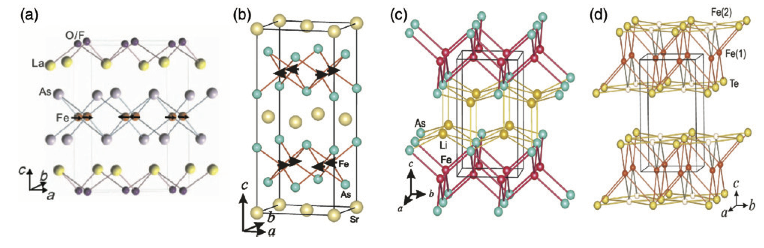
\includegraphics[scale=1.1]{Chapter-Introduction/Figures/PnictideUnitCells/PnictideUnitCells}
        \caption{From left to right: 1111 unit cell, 122 unit cell, 111 unit cell, 11 unit cell. Adapted from ref.~\cite{Johnston2010}}
        \label{Fig:Intro:PnictideUnitCells}
    \end{center}
\end{figure}
The families are labelled according to the ratios of the constituent elements, so for example the `1111' family features four element types in equal proportion, the `122' family features three element types with one of the elements being half as abundant as the other two. In the case of a doped or substituted material, this labelling refers to the stoichiometric parent compound. 

With the exception of the 11 family, the `iron-pnictide' layers are separated by the so called `charge reservoir' layers, which are comprised of a single element type in the case of the `122' and the `111' families and two element types in the `1111' family as shown in figure~\ref{Fig:Intro:PnictideUnitCells}.

Although the highest $T_c$ values have been attained with compounds in the `1111' family (SmFeAsO$_{1-x}$F$_x$ has a $T_c$ of \unit{55}{\kelvin}~\cite{Ren2008}, Gd$_0.8$Th$_{0.2}$FeAsO has a $T_c$ of \unit{56}{\kelvin}~\cite{Wang2008} and Sr$_{1-x}$Sm$_x$FFeAs has a $T_c$ of \unit{56}{\kelvin}~\cite{Wu2009}), it is comparatively difficult to grow large single crystals of the 1111 family causing the emphasis to be shifted to the 11 and the 122 families, especially for neutron scattering studies~\cite{Johnston2010}.

The most studied materials with these transition metal-pnictide/chalcogenide layers typically feature As and P in the pnictide case and Se and Te in the chalcogenide case with the highest $T_c$ values being attained with Fe as the transition metal although superconductivity has been achieved with stoichiometric compounds featuring Ru, Rh, Ir and Ni as the transition metal~\cite{Johnston2010}.



\subsection{Fermiology of the pnictides}

The Fermiology --- i.e. the nature of the Fermi surface --- is key to the formation of the \ac{SDW} state, the onset of which provides the fluctuations necessary for spin-fluctuation mediated pairing and will be described in more detail in the next section. The Bristol group has published a series of results on the Fermiology of various iron-pnictides obtained by \ac{dHvA} measurements which compliment measurements of the Fermi surface by other groups using \ac{ARPES}. A summary of some of these measurements are detailed below.

LaFePO, a member of the 1111 family, has a relatively low superconducting transition temperature of \unit{$\sim$6}{\kelvin}, nonetheless it is a good example to demonstrate the quasi-cylindrical electron and hole Fermi surfaces typical to the iron-pnictides. Figure~\ref{Fig:Intro:PnictideFS} shows the Fermi surface from \ac{DFT} calculations using \ac{GGA} with hole pockets centred around $\Gamma$ and the electron pockets centred around $M$ (adapted from ref~\cite{Carrington2009}).

The momentum separated hole and electron pockets are indicative of a semi-metal, which distinguishes the pnictides from the cuprates\footnote{Cuprates are the other major class of high-$T_c$ superconductors, see section~\ref{Sec:Intro:PhaseDiagram} for an introduction} which are charge insulating antiferromagnets in the undoped state. 

The top right two panels of figure~\ref{Fig:Intro:PnictideFS} shows slices along the 110 plane through the LaFePO \ac{BZ} which demonstrate how the mean field \ac{DFT} calculations had to be adjusted by uniformly shifting the energies in each of the bands to match the \ac{dHvA} measurements. This leads to smaller Fermi surface volumes than the unadjusted \ac{GGA} calculations.

The LaFePO Fermi surfaces are quasi-2D with only relatively weak energy dispersions in $k_z$ which are more pronounced for the electron pockets. In contrast, the middle portion of figure~\ref{Fig:Intro:PnictideFS} shows the Fermi surface for the non-superconducting 122 family iron-pnictide CaFe$_2$P$_2$ measured by the Bristol group~\cite{Coldea2009}. This also demonstrates semi-metal characteristics but a much stronger $k_z$ dispersion leading to entirely 3D hole surfaces. In this case the \ac{GGA} calculations matched the measured \ac{dHvA} data closely with no energy shifts required.
\begin{figure}[htbp]
    \begin{center}
        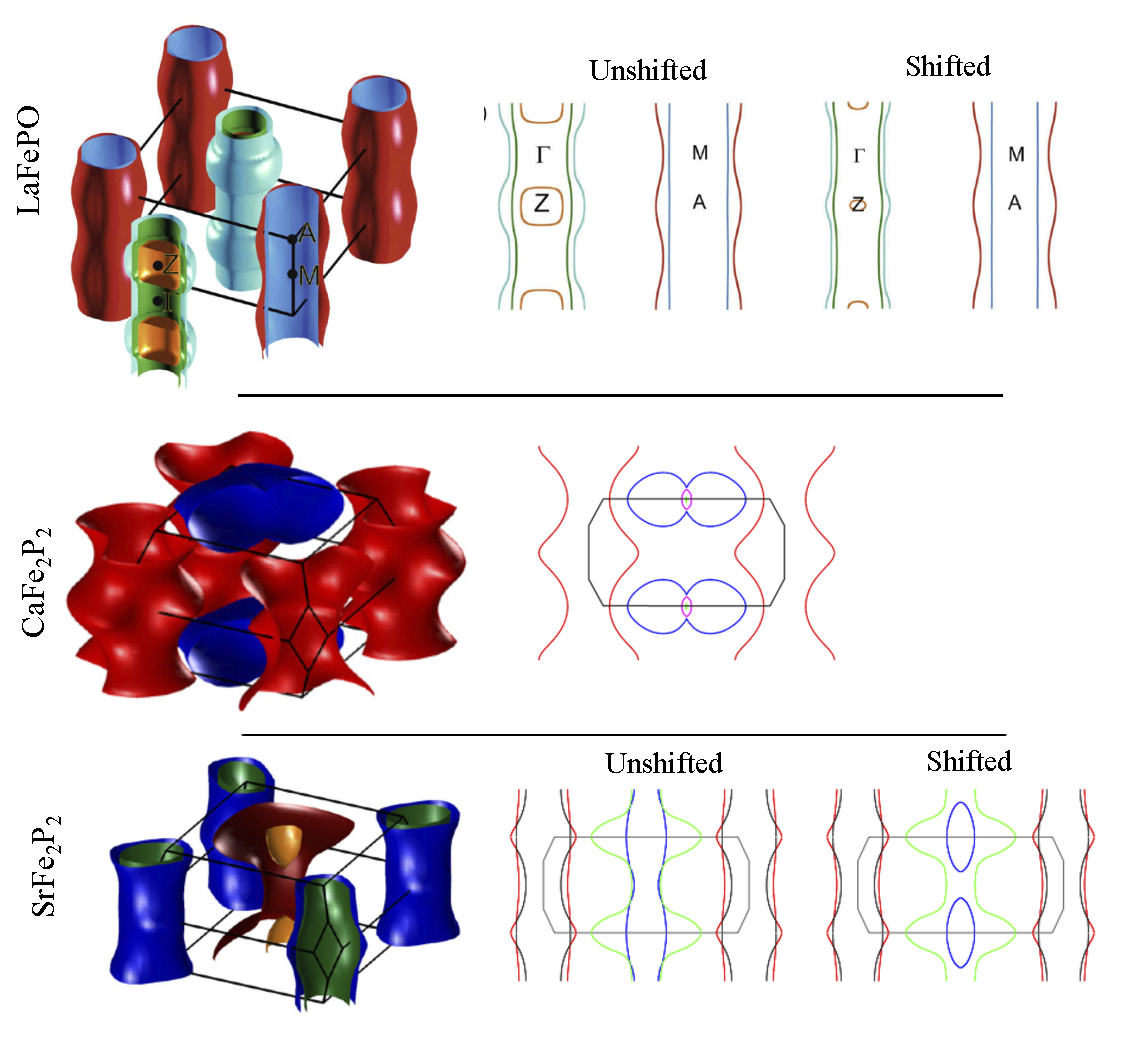
\includegraphics[scale=0.7]{Chapter-Introduction/Figures/PnictideFS/PnictideFS}
        \caption{Fermi surfaces of various iron-pnictides from top to bottom: LaFePO (top) with 110 slices of the \ac{BZ} showing the \ac{DFT} calculations both before (unshifted) and after (shifted) adjustments to match the \ac{dHvA} data. CaFe$_2$P$_2$ (middle) with a 110 slice across the Fermi surface. \SrFeP{} (bottom) with 110 slices similar to LaFePO. Adapted from refs.~\cite{Carrington2009, Coldea2009, Carrington2011, Analytis2009}}
        \label{Fig:Intro:PnictideFS}
    \end{center}
\end{figure}

Comprehensive determination of the Fermi surface of Sr$_2$P$_2$, another non-superconducting 122 phosphide, also shows 3D hole Fermi surfaces as demonstrated in the bottom row of figure~\ref{Fig:Intro:PnictideFS}. In this case it was necessary to shift some of the bands from the \ac{GGA} calculations to match the \ac{dHvA} data. Here the outer hole pocket is strongly warped along $k_z$ but does not pinch off as in the CaFe$_2$P$_2$ case, the inner hole pocket after the shift becomes pinched off and fully 3D.

\SrFeP, CaFe$_2$P$_2$ as well as \BaFeP{} form the end members of superconducting series that begin with the arsenide counterparts. The arsenide parent compound change from the tetragonal structure to an orthorhombic structure below a characteristic temperature, $T_s$ which occurs close to a transition from a paramagnetic phase to a stripe \ac{SDW} state below the N\'eel temperature, $T_N$. This affects the Fermiology by a doubling of the real-space unit cell volume and therefore halving of the \ac{BZ} volume.
\begin{figure}[htbp]
    \begin{center}
        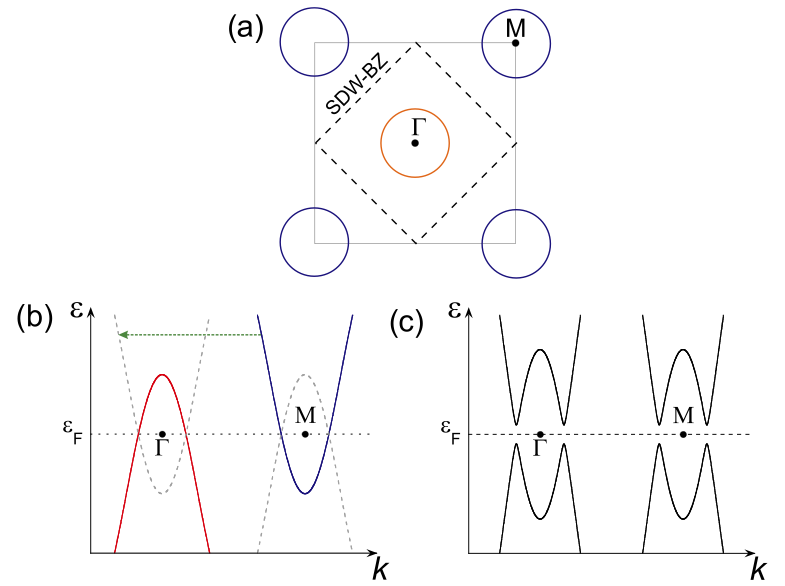
\includegraphics[scale=0.7]{Chapter-Introduction/Figures/AsReconstruction/AsReconstruction}
        \caption{(a) Illustrative 2D projection of the Fermi surface of the tetragonal \ac{BZ} (solid line) with the reconstructed \ac{BZ} as a dashed line (b) Schematic semi-metal band structure of the tetragonal phase showing the hole band at $\Gamma$ and the electron band at $M$ with the dashed lines showing how the folding of the \ac{BZ} aligns the hole bands onto the electron bands (c) The folded \ac{SDW} \ac{BZ} with the resulting gap at the Fermi energy.}
        \label{Fig:Intro:AsReconstruction}
    \end{center}
\end{figure}
The halving of the \ac{BZ} `folds' the larger zone along the dashed lines illustrated in figure~\ref{Fig:Intro:AsReconstruction}~(a) causing the electron bands in the tetragonal \ac{BZ} corners to be superimposed on the hole bands around $\Gamma$ at the \ac{BZ} centre. Figure~\ref{Fig:Intro:AsReconstruction}~(c) demonstrates how the overlaying of the hole and electron bands in momentum space opens a gap around the Fermi energy and the Fermi surface disappears. In practice, the hole and electron Fermi surfaces are not sufficiently symmetric to perfectly cancel and so several small residual hole and electron pockets are left over. \acs{LDA}+U calculations and \ac{dHvA} measurements were performed on BaFe$_2$As$_2$~\cite{Analytis2010b} with the Fermi surface from this publication reproduced in figure~\ref{Fig:Intro:FSBaFeAs}.
\begin{figure}[htbp]
    \begin{center}
        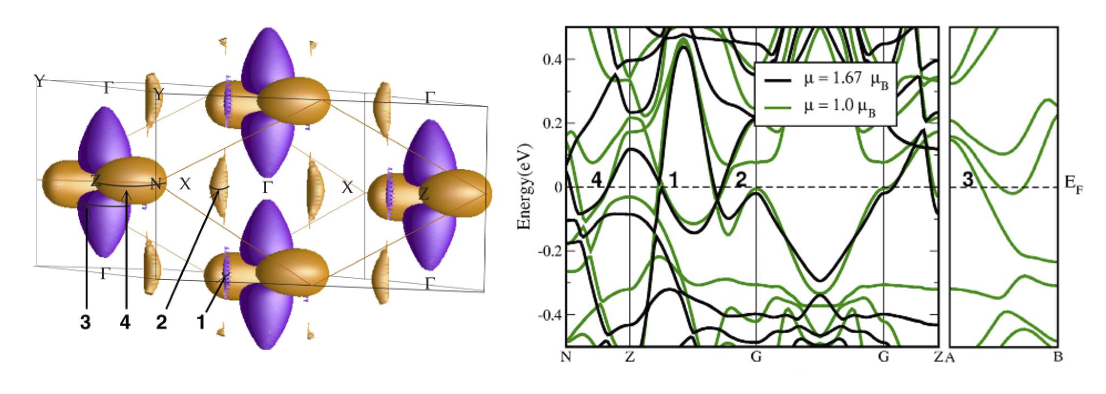
\includegraphics[scale=0.7]{Chapter-Introduction/Figures/FSBaFeAs/FSBaFeAs}
        \caption{Left: BaFe$_2$As$_2$ Fermi surface from \acs{LDA}+U calculations adjusted to fit \ac{dHvA} measurements. Right: Corresponding band structure showing both with (green) and without (black) corrections to $U$.}
        \label{Fig:Intro:FSBaFeAs}
    \end{center}
\end{figure}
Similar measurements were also performed on detwinned\footnote{Similar $a$ and $b$ lattice vectors in orthorhombic crystals can lead to imperfections where one region is rotated by \unit{90}{\degree} with respect to another region. This is known as twinning and when a material which is susceptible to twinning has all the $a$ and $b$ axes aligned, the crystal is said to be `detwinned'.} samples of BaFe$_2$As$_2$ by Terashima \etal~\cite{Terashima2011} which demonstrated similar small pockets with only small difference in detail.


\subsection{The \BaFeAsP{} series}


The \BaFeAsP{} series is one of many that stem from the parent compound \BaFeAs, although unlike the electron doped \BaCoFeAs{} and the hole doped \BaKFeAs{} series, the \BaFeAsP{} progression is entirely isovalent meaning that the changes affected due to the P substitution are due to structure and chemical pressure rather than additional charge carriers. Nonetheless, superconductivity occurs with a very similar phase diagram as with the charge-doped examples in the same $122$ family of iron-pnictide materials.\footnote{See for example figure~1 in ref.~\cite{Paglione2010}}. 

At $x=0$ the \BaFeAsP{} series begins at \BaFeAs, a compound which becomes antiferromagnetic at around \unit{138}{\kelvin}, and moves with increasing $x$ towards \BaFeP{} which is metallic to low temperatures. Neither end members are superconducting, however as As is substituted for P, the low temperature antiferromagnetic state decays, giving way to superconductivity which kicks in at approximately $x=0.18$ and increases to the optimal substitution of $x=0.31$. Superconductivity then decreases until it gives way to a paramagnetic ground state at around $x=0.71$. Figure~\ref{Fig:Intro:PhaseDiagram} shows the phase diagram adapted from ref.~\cite{Nakai2010a} as determined by resistivity measurements. 
\begin{figure}[htbp]
    \begin{center}
        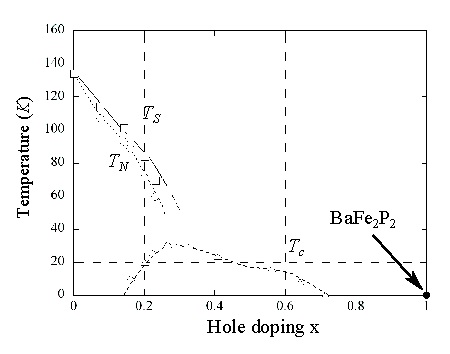
\includegraphics[scale=1.0]{Chapter-Introduction/Figures/PhaseDiagram/PhaseDiagram}
        \caption{Phase diagram adapted from ref \cite{Nakai2010a} measured by resistivity. $T_s$, $T_N$ and $T_c$ are the structural transition, the antiferromagnetic transition and the superconducting transition temperatures respectively.}
        \label{Fig:Intro:PhaseDiagram}
    \end{center}
\end{figure}
Also detailed in the phase diagram is the structural transition which occurs as the tetragonal $I4/mmm$ cell moves to an orthorhombic cell as it passes below the line marked $T_s$. This coincides with the reconstruction of the Fermi surface detailed in the previous section.

 The progression along the series is isovalent since P and As are in the same periodic group -- group $V$. The net effect of the substitution is to apply an increasing chemical pressure as $x$ moves towards $1$. Several reports show that applying high \emph{physical} pressure ($\sim$\unit{5}{\giga\pascal}) to \BaFeAs{} results in a similar phase diagram with an antiferromagnetic phase and superconductivity up to $\sim$\unit{30}{\kelvin}~\cite{Yamazaki2010,Colombier2009,Alireza2009} with Klintberg \etal~\cite{Klintberg2010} presenting a direct comparison between the two types of pressure. As pressure is applied, the unit cell $a$ axis shrinks slightly less than the $c$ axis ($\sim3\%$ cf. $\sim4.5\%$ respectively). Interestingly the $c$ axis shrinking largely occurs in the Fe-Pnictide plane leading to some theories of the superconductivity emerging from the tetrahedral bond angle between the Fe and the pnictogen.
\begin{figure}[htbp]
    \begin{center}
        \includegraphics[scale=1.0]{Chapter-Introduction/Figures/UnitCell/UnitCell}
        \caption{The tetragonal unit cell of the 122 \BaFeAsP{} series clearly showing the tetragonally bonded Fe(As,P) layers.}
        \label{Fig:Intro:UnitCell}
    \end{center}
\end{figure}


The Fermiology of the \BaFeAsP{} series from a substitution of $x=0.41$--$1.0$ has been previously measured by members of the group at Bristol using dHvA oscillations~\cite{Shishido2010}. As suggested in the Shishido reference~\cite{Shishido2010}, since dHvA has been observed across such a large range of substitutions, it implies that the material is not prone to disorder as is the case in many charge doped series~\cite{VanderBeek2010} making the series an excellent candidate for dHvA studies. This could be explained by the fact that the substitution is isovalent and that there is relatively little contribution at the Fermi surface from the pnictide sites\footnote{See for example, the orbital character for the iron sites from \ac{DFT} calculations presented in figure~\ref{Fig:ResD:Band2DCharacterVsKz} in chapter~\ref{Sec:ResD}} where the substitution takes place, meaning the Fermi surface should not be strongly disrupted when traversing the series. The Fermi surfaces from the Shishido paper have been characterised for x ranging from $0.41$ to $1$ for electron sheets only but have clearly shown that the DFT calculations consistently overestimate the size of the surfaces. They also show a linear progression of the electron orbit sizes which is proportional to $x$. Moreover, dHvA measurements on the material with $x=0.63$ have been performed where one of the hole surface extrema was observed~\cite{Analytis2010c} however DFT calculations as well as comparisons with \SrFeP~\cite{Analytis2009} give evidence for a second hole Fermi surface for materials towards the P end of the series, (towards the As end of the series, there appears this second hole and a \emph{third} hole surface similar but smaller to the other hole sheets). If the electron Fermi surfaces are oversized in the DFT calculations, then the hole Fermi surface volumes should also be oversized in order to remain compensated (electrically neutral). What is not clear though is whether the \emph{shapes} of the hole pockets are also altered in the compounds leading to \BaFeP. DFT calculations show the larger of the hole pockets in particular undergoing significant geometric changes, specifically in that it becomes much more three dimensional as P substitution becomes more complete. The Fermi surface of the opposite end-member, \BaFeAs, has been fully characterised by previous \ac{ARPES} measurements~\cite{Kondo2010a} and dHvA~\cite{Terashima2011, Analytis2010b}. Intermediate unreconstructed superconducting compounds have been partially characterised by \ac{dHvA}~\cite{Analytis2010c} and \ac{ARPES}~\cite{Yoshida2010}. Coupled with a full characterisation of the Fermiology of \BaFeP, this unreconstructed Fermi surface data can be used to interpolate Fermiology of the hole pockets across the portion of the phase diagram outside of the \ac{SDW} state.

The \ac{ARPES} measurements of the Fermi surface of \BaFeAs{} below the N\'eel temperature concluded that despite some $k_z$ dispersion in the Fermi surfaces, there is adequate nesting to form the antiferromagnetic state. Ab-initio DFT calculations~\cite{Shishido2010} of the paramagnetic state have shown the $k_z$ dispersion increasing with increasing P, with the outer hole pockets becoming more three-dimensional through the progression providing the partial nesting conditions necessary for pair forming \ac{SDW} fluctuations described in section~\ref{Sec:Intro:Nesting}\footnote{These calculations do not take into account the reconstruction below $T_s$ however for low $x$, and instead assume a hypothetical non-magnetic order.}







\section{The high-$T_c$ pairing mechanism}
\label{Sec:Intro:Nesting}

The previous section details some of the nuances of the cuprate phase diagram but does not make any statements as to what interaction actually causes the Cooper pairs to couple --- the so called `pairing glue'. The second half of this thesis detail measurements which investigate the possibility of \acp{SDW} fluctuations as the bosonic scatterer that bind the electrons together.

The charge carrier in a superconducting condensate is a Cooper pair - a quasi-particle comprising of a bound state of two electrons or two holes with opposite spin and momentum. Evidence for this configuration arises as a natural result of the Ginzberg-Landau model which, when applied to a superconducting system, gives the charge of the quasi-particle carriers as $2e$, where $e$ is the charge of an electron. Given that due to their like charges two free electrons repel, it is natural to ask what could overcome the electromagnetic force to cause these electrons to remain bound in this quasi-particle state.

Bardeen, Cooper and Schreiffer established much of the theoretical basis --- from which the Ginzberg--Landau model can be derived --- in \ac{BCS} \emph{theory} (named after the authors). Within the framework of \ac{BCS} theory, Bardeen Cooper and Schreiffer wrote a 1957 paper~\cite{Bardeen1957} detailed a pairing mechanism known as the \ac{BCS} \emph{model} which would explain how these electron remained bound together. The model is based around the concept of phonons scattering off ions which well suited the superconducting materials known at the time. Phenomenologically, the mechanism of attraction is straightforward. Electrons moving through a crystal lattice attract ions on the lattice sites. These heavy ions respond slowly and are drawn in \emph{behind} the electron. This has the effect of both screening the negative electron charge as well as providing an attractive positive potential for any electron following the original electron. The net effect is the leading electron draws the following electron in its wake, thus coupling them with one another. The wavelike distortion of the ions in the lattice can be considered as a phonon, and the interaction between the electrons and the lattice can be modelled as electron--phonon--electron scattering.

The \ac{BCS} model on top of \ac{BCS} theory accurately describes what we now know as \emph{conventional superconductivity}, that is pairing which forms a spin-singlet state ($S=0$) and which has zero orbital angular momentum ($L=0$). It was not until the discovery of superfluidity\footnote{Superfluidity and superconductivity share much of the same physics although rather than electrons or holes pairing, molecules pair instead. Parallels between the two are discussed in ref.~\cite{Annett2010}} in $^3$He in 1972~\cite{Osheroff1972} that it became apparent that there may exist forms of pairing that resulted in spin-triplet pairing state ($S=1$) with $L>0$. This was later confirmed when superconducting analogues were found in the form of heavy Fermion materials. What really spurred the explosion in interest though was the 1986 discovery by Bednorz and M\"uller~\cite{Bednorz} of high transition temperature (\Tc) superconductivity in the cuprates and, more recently, the `pnictides' by Kamihara et al.~\cite{Kamihara2008}. The cuprate class of materials that Bednorz and M\"uller found to be superconducting have transition temperatures far in excess of any previously known superconducting materials and although the \ac{BCS} model phonon pairing may play a part, the predominant pairing mechanism in the \highTc materials is likely to be something else entirely.

\subsection{The case against conventional superconductivity in high-$T_c$}

There is a great deal of evidence in the literature for non-\ac{BCS} model pairing in the high-$T_c$ and heavy Fermion materials. Although the pairing wavefunction cannot be measured directly with current techniques, experiments indirectly infer \emph{unconventional} i.e. non s-wave, \ac{BCS}-model, characteristics. For example, analysis on penetration depth measurements of \ac{Y123} show power law behaviour~\cite{Annett1991}, indicating that there exists states within the momentum averaged gap. SQUID measurements and Josephson tunnelling experiments on the same material have confirmed alternating phase of the condensate wavefunction which points strongly to \DxTwoyTwo--wave symmetry~\cite{VanHarlingen1994} (see also refs. therein). As for other cuprate materials, specific heat measurements on \ac{BSCO}~\cite{Wang2011}, as well as penetration depth measurements on LSCO~\cite{Froehlich1996} have also proved consistent with $d$-wave pairing. 

More evidence against conventional superconductivity include the unusual normal state (i.e. non-superconducting) state properties of the cuprates and heavy Fermion materials. The \ac{BCS} model is grounded in Landau Fermi liquid theory which models interacting itinerant electrons with quasiparticles of heavier effective mass than ordinary electrons and holes. A hallmark of Fermi liquid behaviour is a $T^2$ dependence of the resistance, however experiments on the cuprate \ac{LSCO}~\cite{Cooper2009} and a heavy Fermion material~\cite{Custers2003} have demonstrated fractional power law behaviour, $T^\gamma$ where $1 < \gamma < 2$, at temperatures above the superconducting transition. Given that the Fermi liquid model breaks down in these examples, it follows that the \ac{BCS}-model also is likely on shaky ground for these materials.

There are several arguments against phonons as the sole pairing mechanism in the pnictide case, Boeri et al.~\cite{Boeri2008} and Mazin et al.~\cite{Mazin2008} present calculations showing that the magnitude of the phonon pairing strength is not adequate for the high \Tc values attained in LaAsOF, Haule et al.~\cite{Haule2008} note in the same material that the gradient of the density of states (DOS) at the Fermi level is such that you would expect an increase in DOS and hence \Tc with hole doping if the \ac{BCS} model held, however the reverse is true. Non Fermi-liquid behaviour was demonstrated in the \BaFePAs series~\cite{Jiang2009,Kasahara2010} and although many superconducting pnictides are believed to have a nodeless superconducting gap~\cite{Hashimoto2012,Zhang2011a,Ding2008, Terashima2009} there are many~\cite{Fletcher2009, Qiu2011b, Song2011, Dong2010, Hashimoto2012} including the \BaFePAs series~\cite{Zhang2011,Yamashita2011a,Suzuki2011} which are thought to have nodes.

It is interesting to note that unlike the cuprates which universally show a \DxTwoyTwo gap symmetry, the pnictide materials are note all alike, even pnictides along the same series such as the LiFeAs and LiFeP show a change in gap structure. Consequently, it may prove that the nature of the superconductivity may not be universal amongst the pnictide materials. Irrespective of this, the \ac{BCS} model pairing alone has been shown to be too weak to explain high-$T_c$ superconductivity.


\subsection{Spin-fluctuations}

One possible alternate pairing mechanism arises from scattering due to spin fluctuations. A common feature of phase diagrams for all of the pnictides and the cuprate materials is close proximity of a \ac{SDW} magnetic state to the superconducting state.
\begin{figure}[htbp]
    \begin{center}
        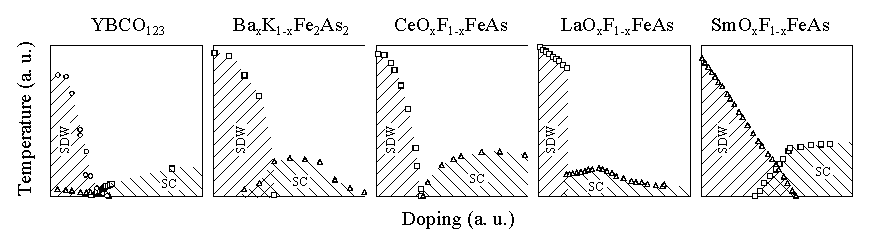
\includegraphics[scale=1.0]{Chapter-Introduction/Figures/PhaseDiagrams/PhaseDiagrams}
        \caption{Phase diagrams for various \highTc materials adapted from ref.~\cite{Uemura2009} showing the proximity of the superconducting phase (SC) to the spin density wave state (SDW) in all cases}
        \label{Fig:Theo:PhaseDiagrams}
    \end{center}
\end{figure}
As described in more detail in section~\ref{Sec:Theo:SpinDensityWave}, the \ac{SDW} state is a general form of magnetic order that describes a periodic modulation of the spins of a system and encompasses antiferromagnetism and arguably ferromagnetism. As a system enters a \ac{SDW} state, short range, damped, antiferromagnetic fluctuations occur and it is these that are thought to provide the pairing interaction for the Cooper pair states.

Spin fluctuations were originally investigated as a mechanism which \emph{suppressed} conventional, i.e. $s$-wave, superconductivity~\cite{Berk1966} from ferromagnetic fluctuations and were used to explain why nearly ferromagnetic metals such as Pd has lower than expected $T_c$. Later however it was found that for symmetries such as $d$-wave that \emph{antiferromagnetic} spin fluctuations could possibly provide an interaction which is attractive and could overcome the Coulomb repulsion~\cite{Scalapino1995}.

Typically spin-fluctuations occur due to favourable band structure conditions, in particular where there is a \emph{nesting} condition. This is where a hole-like Fermi surface band maps through reciprocal space onto a similarly sized electron-like Fermi surface via a particular vector $\vect{q}$ known as the nesting vector. Since strong nesting leads to a stable \ac{SDW} state, we are looking for only partial nesting in the Fermi surface of superconducting materials so that we get enough spin fluctuations to cause pairing but not too many to cause a full \ac{SDW} state.

As an aside, nesting is not the only cause of spin fluctuations. For example, frustrated spin systems such as the Kagome triangular lattice can also be a cause of spin fluctuations, however this is thought to occur only in very specific 1D and 2D materials.

\subsection{Pairing in the pnictides}

Soon after the discovery of the pnictide materials, a possible pairing mechanism was proposed based on on the above described spin density wave fluctuations. The original paper suggested a $s_{\pm}$ gap symmetry~\cite{Mazin2008} which features a multi band model based on LaFeAsO$_{1-x}$F$_x$. The spin fluctuation coupling vector couples over the \ac{BZ} diagonal two separate, approximately cylindrical, Fermi surfaces of opposite phase. Although this is an extended $s$-wave model, the geometry is satisfied by the relative positions of the Fermi surfaces within the \ac{BZ}. 

As already stated, more recent measurements have discovered nodes in the gap structure in many pnictide materials and while no nodes featured in the original Mazin model, there is no reason why the model can be adapted to include them.

% \TODO{What actually is the cause of the attraction in the nesting picture? ... Spin fluctuation interaction in real space is approximately proportional to the dipole interaction $V=-\mu . \mu \chi(r)$}%\cite{Bergemann2003}

% Strong correlations - the interaction energy is much greater than the kinetic energy for the states
% When correlations present, Cooper pairs are assumed to be pairs of Landau quasiparticles

% The Stoner condition of $\mathcal{N}_0 I > 1$ -- where $\mathcal{N}_0$ is the density of states at the Fermi energy and $I$ is the molecular field constant, that scales the magnetism given a field -- indicates an energy instability\cite{Kubler2000}



\section{The cuprate phase diagram}

The phase diagrams for the \highTc materials show a remarkable consistency across the cuprates\footnote{This is in contrast with the recently discovered pnictide materials which show significant variations in scalings and even composition}. However this universality amongst the cuprates comes with an abundance of features which provide for some complex physical interactions and fragile intermediate `crossover' phases. The tuning parameter for the cuprate phase diagram is either electron or hole doping typically performed by elemental substitution at the crystal growth stage or by oxygen incorporation through annealing. As shown in figure~\ref{Fig:Intro:ElecHolePhaseDiagram}, the two types of doping are not symmetric with hole doping generally resulting in more robust superconductivity. For this reason the literature has largely concentrated on the hole doped progression and as a result it is far better characterised. The doping is usually expressed as a $p$ value which represents the amount of additional holes (electrons) per Cu atom.
\begin{figure}[htbp]
    \begin{center}
        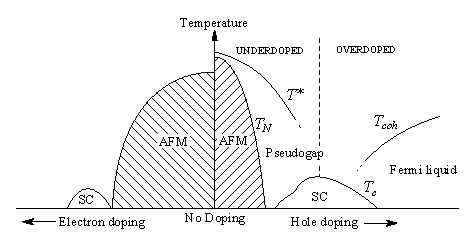
\includegraphics[scale=1.0]{Chapter-Introduction/Figures/ElecHolePhaseDiagram/ElecHolePhaseDiagram}
        \caption{A schematic phase diagram showing electron doped to the left and hole doped to the right. \ac{AFM} is the antiferromagnetic Mott insulating phase, SC is the superconducting phase. $T^*$, $T_N$, $T_c$ and $T_{\textrm{coh}}$ are the temperature scales for the pseudogap, \ac{AFM} state, superconductivity and coherent Fermi liquid phases respectively}
        \label{Fig:Intro:ElecHolePhaseDiagram}
    \end{center}
\end{figure}

\subsection{Mott insulating parent compound}

Starting at the middle of figure~\ref{Fig:Intro:ElecHolePhaseDiagram}, the parent compound materials at zero doping are thought to be Mott insulators i.e. the top most filled state on each lattice site contains one electron. In the conventional band picture this should be metallic since the bands are only partially filled, however when we consider a local picture of electrons, any movement of an electron to the neighbouring lattice site will cause an energetically costly double occupancy on one site and zero occupancy on another. This causes the electronic \ac{DOS} to become gapped around the Fermi surface and hence suppressed conduction. This is known as the Mott insulating state.

We find that the kinetic energy term is reduced when the ordering of the sites is antiferromagnetic since for any hopping to occur at all, the spins must be antialigned to avoid double occupancy of like spins. This region dominates the low doping portion of the phase diagram and remains antiferromagnetic until either the temperature is high enough to allow transitions from the Fermi energy to the states at the edge of the gap or the doping has introduced enough double occupancy electrons on lattice sites, which can move without the double occupancy energy cost, to overcome the insulating behaviour.

\subsection{Superconducting dome}

With increased doping, the antiferromagnetic state gives way to the superconducting dome at around $p=0.05$ which itself gives way to a Fermi liquid metallic state at a doping of around $p=0.3$. The maximum \Tc occurs at around $p=0.16$. Transitions from both the antiferromagnetic and the superconducting state are clearly second order thermodynamic with jumps in the heat capacity for example, however there are other regions in the phase diagram which are less well defined such as the pseudogap and the Fermi liquid crossover whose temperature scale can depend on the particular probe used and do not feature a clear order parameter.

\subsection{Coherent phase}

To the heavily overdoped side of the phase diagram, beyond the superconducting dome lies the coherent region where the system bears the hallmarks of a conventional metal. The implication is that correlations between electrons are sufficiently weak such that the mass enhanced quasiparticles of Landau's Fermi liquid theory are well defined, leading to conventional metal behaviour. A clear indication of this is a dominant $T^2$ term in the resistivity. Above this region we observe an anomalous additional contribution which has been modelled both with $T^2$ plus an additional linear term or by a $T^n$ term where $1 <= n <= 2$. This additional term has been observed in heavy Femrion materials and is often associated with proximity to a \ac{QCP}~\cite{Custers2003}.

\subsection{The pseudogap}

Above the antiferromagnetic region and the superconducting state is one of the most controversial regions of the phase diagram, the so called pseudogap phase. This is a region which was first demonstrated in 1989, just a few years after the discovery of the cuprate materials, by \ac{NMR} measurements performed at Bell labs~\cite{Warren1989}. A noticeable fall in the susceptibility occurred at a temperature significantly above $T_c$ which led to conclusion of possible spin pairing before the onset of bulk superconductivity\footnote{Cooper paired electrons in the singlet state have zero net spin hence they do not contribute to the susceptibility, whereas unpaired electrons do. Cooper pairing leads to a reduction in susceptibility, see for example neutron scattering plots.}. The question arose as to what the exact relation of the pseudogap is to the superconducting state --- is it a precursor state, from which superconductivity arises or is it a competing phase? --- and from a materials development point of view, to obtain higher $T_c$ should we be finding ways to suppress the crossover to the pseudogap state or encourage it?
\begin{figure}[htbp]
    \begin{center}
        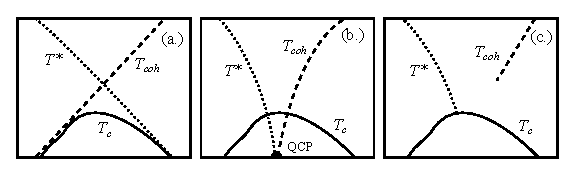
\includegraphics[scale=1.0]{Chapter-Introduction/Figures/PGScenarios/PGScenarios}
        \caption{Three scenarios proposed for the $T^*$ temperature scale behaviour. (a.) the pseudogap as the `precursor' state, (b.) as the `competing' state, (c.) and the `transition' scenario.}
        \label{Fig:Intro:PGScenario}
    \end{center}
\end{figure}
By finding where exactly the $T^*$ energy scale meets the superconducting dome, strong evidence can be found that supports one or the other scenario. However the problem lies in the type of probe used. Select spectroscopic measurements including \ac{STM}, \ac{ARPES} and Raman spectroscopy on materials of comparable $T_c$ values have found that the $T^*$ overreaches the superconducting dome entirely~\cite{Hufner2008}, meeting with the overdoped edge at $T=\unit{0}{\kelvin}$. This supports the precursor state theory illustrated in figure~\ref{Fig:Intro:PGScenario}~(a.) where $T^*$ and $T_{\textrm{coh}}$ cross to define a region which is below both temperature scales where the carrier are both coherent quasiparticles and paired leading to the superconducting condensate.

A second scenario is supported by measurements using bulk probes such as heat capacity, magnetic susceptibility and resistivity measurement have shown the $T^*$ energy scale drops into the top of the superconducting dome~\cite{Tallon2001}. This supports the scenario where the pseudogap is in competition with superconductivity for states at the Fermi surface. Once the pseudogap phase is suppressed, scattering from quantum fluctuations at zero temperature leads to the formation of the superconducting phase at a \ac{QCP} similar to that found in heavy fermion materials. This scenario is supported by the observation of linear scaling of the resistivity with temperature in the region above the superconducting dome which is a hallmark of proximity of a \ac{QCP}.
% Kondo is a competitive scenario which justified based on
% non-monotonicity of coherence as you move from the antinodes on the FS \cite{Kondo2009}

A third scenario is one where the pseudogap simply becomes the superconducting gap as it meets the top of the superconducting dome. However this scenario leaves hanging questions as to the roles of the pseudogap, $T_{\textrm{coh}}$ and other phenomena in the phase diagram which would need to be addressed theoretically. Moreover this picture is rendered less compelling by the observation in \ac{LSCO} of rapidly increasing, low temperature, normal state resistivity inside of the underdoped superconducting dome which implies the non-superconducting energy gap persists into this region.


\subsection{Previous work by the Bristol group}

Clearly lots of interesting physics is occurring in and around the superconducting dome and a solid understanding of this region is key to understanding the problem of high-$T_c$. Prof. N. Hussey has been involved in many efforts to shed light on the situation, of which, two key ones are highlighted here.

\subsubsection{Links between anisotropic scattering and $T_c$}

Simply measuring resistance along different axes gives an averaged scattering rate through all conduction paths and so to build a map of the angle dependent scattering rates, a different technique must be used. In \ac{ADMR} a strong persistent magnetic field is applied before resistance measurements are taken. The field serves two purposes; firstly, to suppress superconductivity so the normal state can be probed, secondly to confine the electrons to orbits perpendicular to the field. By detailed analysis of the change in resistance as the field is applied at various angles, a picture of the angle dependent scattering rate can be determined.

After performing measurements on samples of \ac{TL2201} with dopings ranging from strongly overdoped to slightly underdoped~\cite{Abdel-Jawad2006}, a trend emerged which is illustrated in figure~\ref{Fig:Intro:AnisotropyPhase}. 
\begin{figure}[htbp]
    \begin{center}
        \includegraphics[scale=0.9]{Chapter-Introduction/Figures/AnisotropyPhase/AnisotropyPhase}
        \caption{Schematic of how the scattering rate, $\Gamma$, the Fermi surface, $FS$, and the superconducting gap, $\Delta_g$ evolve with doping across the superconducting dome. Based on figure 1 in ref~\cite{Taillefer2006}. The dotted line in the scattering is the isotropic part.}
        \label{Fig:Intro:AnisotropyPhase}
    \end{center}
\end{figure}
Here the scattering rate within the $ab$-plane, $\Gamma$, was found to be composed of two terms; an isotropic term which remained constant with doping (dotted circle) and an anisotropic component which scaled with the superconducting gap, $\Delta_g$. Moreover it was found that the superconducting gap and the anisotropic scattering rate both shared the same shape, being `d-wave'. This further ties to \ac{ARPES} measurement which show that the on the underdoped side of the superconducting dome there is a pronounced change in the Fermi surface where at the antinodal points of $\Gamma$ (and $\Delta_G$) the spectral weight disappears~\cite{Norman2010} i.e. coherent particles are lost away from the regions of strong scattering.

%It changes from a single large hole band of volume $1+p$ to series of small regions of electron and hole Fermi surface of total volume $p$.

\subsubsection{T-Linear behaviour in the superconducting dome}

Previous high-field transport measurements on Sr doped \ac{LSCO}~\cite{Cooper2009} gave key insights into the nature of the T-linear term as it entered the superconducting term on the overdoped side. In particular it showed that the T-linear term did not funnel down to a point (figure~\ref{Fig:Intro:CooperTLinear}) as is typical of \ac{QCP} behaviour but instead spread out into the superconducting region. Intrigued as to this unexpected behaviour, we looked to repeat the measurements on \ac{BSCO} which can be doped far more widely without divergence in the resistivity so that we could then see how the T-linear term progressed on the underdoped side, where $T^*$ is undisputed.
\begin{figure}[htbp]
    \begin{center}
        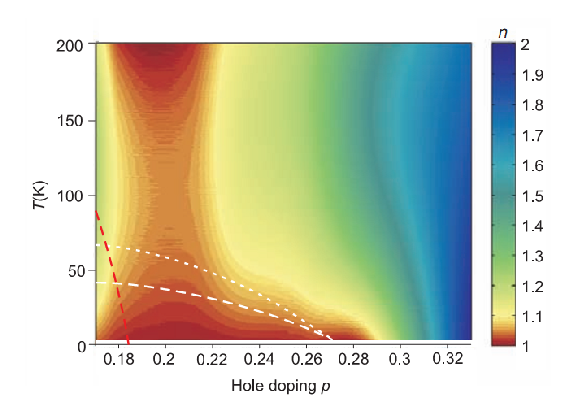
\includegraphics[scale=0.8]{Chapter-Introduction/Figures/CooperTLinear/CooperTLinear}
        \caption{Plot of the $T^n$ term in the fitted field suppressed normal state of Sr doped \ac{LSCO} showing the $T$-linear term extending throughout the superconducting dome and not to a single \ac{QCP}. Taken from Cooper \etal~\cite{Cooper2009}}
        \label{Fig:Intro:CooperTLinear}
    \end{center}
\end{figure}
Performing measurements which would shed light onto which of the scenarios shown in fig~\ref{Fig:Intro:PGScenario} is most likely to be correct formed the original motivation for the investigation of \ac{BSCO} through transport measurements. 

A second reason for the study of \ac{BSCO} in particular is that it's van-Hove singularity occurs at a different doping --- further from optimal doping --- than \ac{LSCO}. Should similar behaviour be found then we can confidently claim that the unusual \ac{QCP} behaviour is not due to proximity to the changeover in hole-like to electron-like Fermi surface and is likely universal to all cuprates. 

\ac{BSCO} also demonstrates transport behaviours which are consistent with other high-$T_c$ cuprate materials. For example, from \ac{MR} measurements it demonstrates a similar maximum in the underdoped $d\rho_{ab}/dT$ curve as underdoped YBCO~\cite{Ando1999}. On the overdoped side, \ac{BSCO} demonstrates a monotonic upward trend in $d\rho_{ab}/dT$ with increasing temperature similar to what has been observed in Tl$_{2201}$ and \ac{LSCO}~\cite{Ando1999}.

During the course of the investigations however, it became apparent that even with field strengths of up to \unit{60}{\tesla} in pulsed fields, the upper critical field, $H_{\textrm{c2}}$ of many of the sample at key temperatures could not be reached. However, field strengths were generally strong enough to recover $B$-Linear behaviour in the Hall component.

Previous Hall measurements have been performed on \ac{BSCO} by Ando \etal~\cite{Ando1999, Ando2000} which are shown for comparison in the results section. However these results do not go to low temperatures, being restricted by the onset of superconductivity. Our own results used high field measurements at \ac{LNCMI} and \ac{HFML} to suppress superconductivity and examine the low temperature regions in detail. Moreover our samples are focused on the overdoped region which complements the underdoped data set presented in the Ando papers.

% Motivation

% Lograithmic divergence of scattering rate observed in cuprates which
% begins at critical doping and increases as become more underdoped.
% However common factor of cuprates (Y123, Tl2201, LSCO) is a change of
% Fermi surface (in LSCO at least) from hole to electron leading to a
% van Hove singularity(?) which occurs similar to hwere would expect the
% insulating crossover. This does not occur in BSCO however until
% around p=0.2\cite{Hashimoto2008}. If the \alpha^2 term takes off
% earlier for BSCO\cite{Hussey2011a} is good
% evidence that is due to the proximity to van Hove rather  than Moot
% insulator transition.\cite{Ono2000}


% \section{Mott physics}

% The Hubbard model takes the relatively simple and solvable tight-binding model and introduces an Anderson term which raises the energy for double occupancy by an amount $U$, known as the `Hubbard U'. This simple change deeply enriches the physics with one of the outcomes being the existance of the Mott insulating state which occurs when each lattice site is half filled with a single electron. The energy cost for an electron to hop to an adjacent site is so high that it locks the electrons in place, preventing effective conduction. Introducing holes (or electrons) allows once again hopping to take place and the eigenstates are no longer entireley localised.



\subsection{Properties of \acs{BSCO}}

The unit cell of the \highTc, doped cuprate \acf{BSCO} is illustrated in figure~\ref{Fig:Intro:BSCOUnitCell}. It is made up of layers as follows from the top; a BiO layer, then a SrO layer, then a CuO lattice common to all cuprates, then 2 BiO layers, a SrO layer, CuO, SrO, BiO. Variants of \acs{BSCO} include \ac{BSCO2212} and \ac{BSCO2213} which feature one and two extra CuO layers respectively. Most closely relatated in terms of structure is \acs{TL2201} which features Tl and Ba in place of Bi and Sr repsectivey.
\begin{figure}[htbp]
    \begin{center}
        \includegraphics[scale=1.1]{Chapter-Introduction/Figures/BSCOUnitCell/BSCOUnitCell}
        \caption{Unit cell of \acs{BSCO} demontrating the layers. \ac{TL2201} is similar but with La for Bi and Ba for Sr. Note that Pb doping occurs away from the CuO planes.}
        \label{Fig:Intro:BSCOUnitCell}
    \end{center}
\end{figure}
Undoped \ac{BSCO} has an excess of holes and lies slightly to the undoped side of the phase diagram. By substituting in La for Sr, the amount of holes is reduced allowing access to a range of slightly overdoped to underdoped. However, since the substitution takes place adjacent to the CuO planes where all the interesting electronic behaviour happens, La doping introduces a lot of disorder into the system. Pb is also substituted for Bi which increases the number of holes alowing the more overdoped region to be accessed. Since Pb substitutes into the BiO layer which is far from the CuO plane, less disorder is introduced. Sometimes Pb is introduced alongside La even when a more underdoped state is desired to avoid forming structures in the BiO planes which affect \ac{ARPES} measurements~\cite{Kondo2007}. Furthermore, annealing in oxygen decreases the number of carriers depending on how much additional oxygen is obsorbed allowing for even more fine grained tuning of the doping. By adjusting these parameters a very wide range of doping values can be accessed in \ac{BSCO} which makes it appealing for study.

The precise determination of doping from a chemical standpoint is tricky. For \ac{LSCO} --- assuming pure ionic donation --- substituting more Sr for La simply adds one more hole per extra Sr atom per unit cell. However for \ac{Y123} and \ac{Y124} for example, tehre exist CuO chains (oxygen deficient CuO layers) which absorb some of the doped charge, other cuprates the heavy metal atom has a mixed valency meaning that the substitution relation is not so straightforward. Various techniques described in the methods section have been described to determine the doping level but as a rule some a priori knowledge of composition is required.
\begin{figure}[htbp]
    \begin{center}
        \includegraphics[scale=0.9]{Chapter-Introduction/Figures/VanHoveBSCOLSCO/VanHoveBSCOLSCO}
        \caption{Band dispersions at the Fermi energy for various dopings. Left panel shows \ac{BSCO}, right panel shows \ac{LSCO}. Note the saddle points at $(\pi, 0)$ which cause the van-Hove singularity at $p\approx 0.18$ for \ac{LSCO} and at $p \geq 0.2$ for \ac{BSCO}. Adapted from ref~\cite{Hashimoto2008}.}
        \label{Fig:Intro:VanHoveBSCOLSCO}
    \end{center}
\end{figure}
There is a crossover in overdoped curpates between a large hole-like Fermi surface to an electron-like Fermi surface that leads to a saddle point in the \ac{DOS} and consequently a van Hove singularity (see figure~\ref{Fig:Intro:VanHoveBSCOLSCO}, adapted from ref.~\cite{Hashimoto2008}). This occurs in \ac{LSCO} at around $p=0.18$ which is approximately critical doping and may lead one to believe that the critical behaviour is related to the proximity of the van Hove singularity. However the same crossover does not happen at the same doping in \ac{BSCO}, rather it appear to occur at $p \geq 0.2$, relatively far fromt he critical value of $p \approx 0.16$. For this reason \ac{BSCO} is an attractive material to study to determine more about the relationship (or lack thereof) between the critical behaviour and the van Hove singularity.

Finally \ac{BSCO} has a relatively low maximum \Tc, being around \unit{36}{\kelvin} at best. Because \Tc is so low, this makes \ac{BSCO} idealf or normal state study since less field will be required to suppress \Tc at lower temperatures.



